% !TEX root = ./problem.en.tex
\gdef\thisproblemauthor{}
\gdef\thisproblemdeveloper{}
\gdef\thisproblemorigin{}
\begin{problem}{魔樹 OldTree}
{standard input}{standard output}
{2 seconds}{512 MB}{}

傳說,在府城第零高級中學中央的大榕樹擁有強大的魔性\newline
校園裡也因此流傳著許多圍繞著大榕樹的傳說 -- 那些人們不以為意的事\newline
然而那一天,人類回想起了,一度被支配的恐懼...\newline
\newline
2087年8月7日 晚間 8點07分\newline
他,再次甦醒了\newline
其盤根汲取生命,其枝葉揮舞恐懼,其果實凝結黑暗...\newline
人類的力量在其面前顯得微不足道\newline
然而,希望的光芒並沒有消滅\newline
人們找到了削弱他力量的方式 -- 斷根\newline
\newline
大榕樹的根盤據各處,有些根會交在一起,形成一個可以儲存生命力的樹瘤,每個樹瘤儲存的生命力多寡不一,透過切除樹瘤就能削弱大榕樹的生命力。當切除一個樹瘤後,有些其他樹瘤可能因此不再和樹幹間接相連,這些樹瘤也就視同被切除了。\\
\newline
先遣的調查隊已經整理出所有樹瘤的連接關係:\newline
以編號 $1 \sim N$ 表示 $N$ 個樹瘤,編號 0 則表示大榕樹的樹幹\newline
以 $M$ 個整數對 $(a,b)$ 表示編號 $a$ 和 編號 $b$ 之間有樹根直接連接\\
\newline
切除樹瘤必須冒險進入大榕樹的攻擊範圍內,所以只能切一個,請根據這些連接關係找出,切除後能讓大榕樹減少最多儲存生命力的樹瘤吧!\newline


\InputFile

第 1 行:2個正整數 $N$,$M$ (空白分隔) ,表示有 $N$ 個樹瘤、$M$ 個連接關係 \newline
第 2 行:$N$ 個正整數 $v_1,v_2,...v_N$ ,表示編號 $1 \sim N$ 的樹瘤分別存有多少生命力 \newline
第 3 行以後:$M$ 對正整數 $a,b$ (空白分隔,每對佔一行) \newline
                      表示 編號 $a$, 編號 $b$ 之間有根直接相連接  \newline

\begin{iofmt}
\begin{itemize}
	\item $1 \leq N \leq 10^5$
	\item $M \leq \frac{{}(N+1) \times N}{2},\ M \leq 10^6$
	\item $0 \leq a, b \leq N,\ a\neq b$
	\item $v_i \leq 10^4$
	\item 一筆測資中不會有完全相同的兩對 $(a,b)$
	\item 所有樹瘤都與樹幹直接或間接相連
	\item 有 36 分的測試資料 $M = N$
	\item 有 36 分的測試資料 $N \leq 1000$
\end{itemize}
\end{iofmt}

\OutputFile

輸出一個正整數,表示消去後可以讓大榕樹損失最多生命力的樹瘤的編號 \newline
若有多個樹瘤都能達到同樣的效果,則輸出編號最小的 \newline

\Examples

\begin{example}
\exmpfile{./sample/PC-01.in.txt}{./sample/PC-01.out.txt}%
\exmpfile{./sample/PC-02.in.txt}{./sample/PC-02.out.txt}%
\end{example}

以下為第一筆範例的說明\\
\\
原貌:\\
\centerline{ 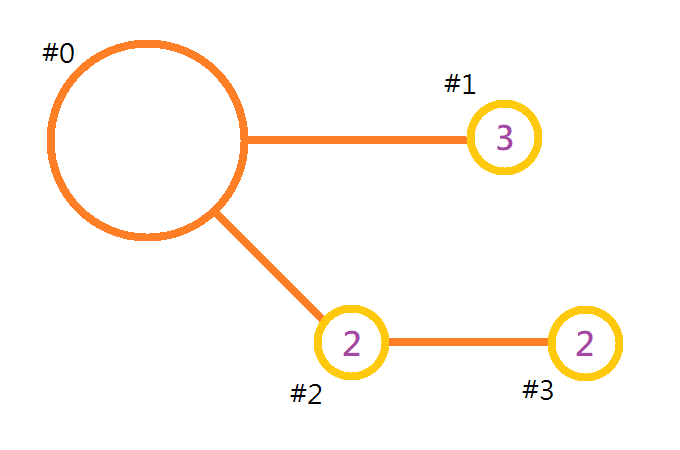
\includegraphics[scale=0.5]{./pics/C-1.png} }
拔除 編號2:\\
\centerline{ 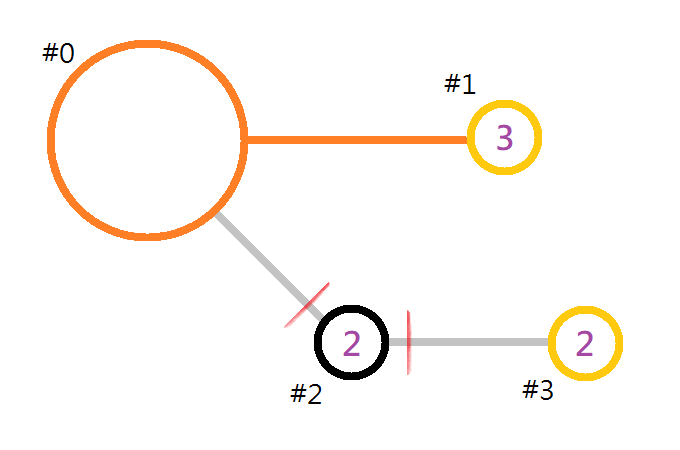
\includegraphics[scale=0.5]{./pics/C-2.png} }
拔除 編號 2 之後,編號 3 也被隔開了,只剩下 編號1 連接著\\
\centerline{ 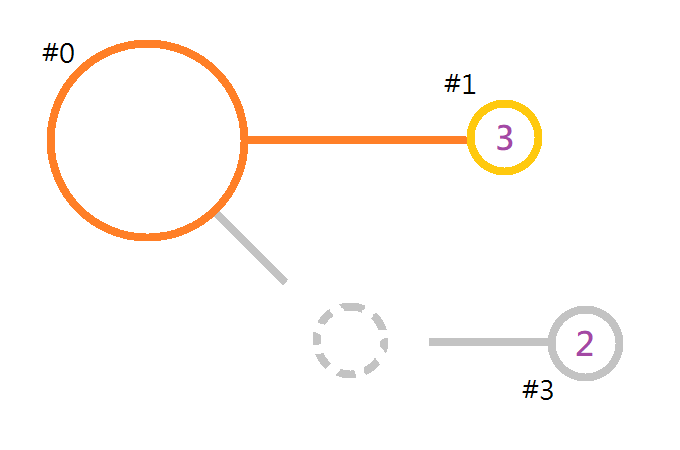
\includegraphics[scale=0.5]{./pics/C-3.png} }

\end{problem}
